\section{Advanced topics}

In many processes of interest in practical problems, the strict assumptions of a linear system with Gaussian process and measurement noise are not satisfied.
For instance, consider the radar tracking problem: radar will usually measure the range and bearing and elevation angles to a target.
The measurement noise is not likely to be perfectly Gaussian.
One can either write the target dynamic equations in terms of range and angles (in which case the dynamics are nonlinear); or, one may compute 3-dimensional coordinates $x,y,z$ from the raw measurements, in which case the measurement noise undergoes a nonlinear transformation.
There is no perfect general transformation that allows the strict assumptions of linear dynamics and linear measurements to be guaranteed. This motivates the need for nonlinear estimators.

Perhaps the most intuitive approach to the nonlinear estimation problem is to linearize the nonlinear system about the prior state, and use the Jacobians of the system in the Kalman covariance equations.
This process is the EKF, and is widely used for nonlinear estimation in many fields including aerospace and process engineering.
The linearized approximation, however, may fail in some cases, particularly if an accurate prior for the estimate is not known.
This has motivated the developement of other techniques.
The UKF, sometimes called the Sigma Point Filter, uses a discrete approximation to the prior density.
The literature indicates that this approximation is more accurate than the linearization of the EKF \cite{wan2000}.
The remainder of this section presents an overview of the EKF and UKF.
We begin with a presentation of the EKF.

\subsection{Extended Kalman Filter}

This discussion is motivated by Ref. \cite{crassidis2011}.
Consider a generic discrete nonlinear system with discrete nonlinear measurements and discrete controls $\vecin{u}{k}$, and a Gaussian prior for the estimated state.
Let $\vecin{w}{k}$ and $\vecin{v}{k}$ indicate zero-mean process noise and measurement noise:
\begin{equation}
\vecin{x}{k+1} = \f(\vecin{x}{k},\vecin{u}{k}) + \G(k) \vecin{w}{k}
\end{equation}
\begin{equation} \vecin{y}{k} = \h(\vecin{x}{k}) + \vecin{v}{k} \end{equation}
\begin{equation} E[\vecin{x}{0}] = \vecin{\hat{x}}{0} \end{equation}
\begin{equation} var[\vecin{x}{0}] = \P(0) \end{equation}
\begin{equation} E[\vecin{w}{k}] = 0\end{equation}
\begin{equation} var[\vecin{w}{k}] = \ten{Q(k)}\end{equation}
\begin{equation} E[\vecin{v}{k}] = 0\end{equation}
\begin{equation} var[\vecin{v}{k}] = \ten{R(k)}\end{equation}

In general, the MMSE for the nonlinear system is intractable \cite{kay1993}.
An approximate solution can be obtained by linearizing the nonlinear governing equations, sacrificing the optimality properties of the linear KF.
A brief summary of the derivation of the EKF equations is presented.
Let $\vecin{\hat{x}}{k}$ denote the (prior) estimate of the state at time step $k$ and $\vecin{x}{k}$ denote the unknown true state.
The nonlinear functions can be expanded in two terms of a Taylor series approximation as follows:

\begin{equation}
\f(\vecin{x}{k},\vecin{u}{k}) \approx \f(\vecin{\hat{x}}{k},\vecin{u}{k}) + \ddarg{\f(\vec{x},\vecin{u}{k})}{\vec{x}} \pip_{\vec{x}=\hat{x}_k} (\vecin{x}{k}-\vecin{\hat{x}}{k}) \end{equation}
\begin{equation}
\h(\vecin{x}{k}) \approx \h(\vecin{\hat{x}}{k}) + \ddarg{\h(\vec{x})}{\vec{x}} \pip_{\vec{x}=\vecin{\hat{x}}{k}} (\vecin{x}{k}-\vecin{\hat{x}}{k}) \end{equation}
\begin{equation}
\F(k) \equiv \ddarg{\f(\vec{x},\vecin{u}{k})}{\vec{x}} \pip_{\vec{x}=\vecin{\hat{x}}{k}} \end{equation}
\begin{equation}
\H(k) \equiv \ddarg{\h(x)}{\vec{x}} \pip_{\vec{x}=\vecin{\hat{x}}{k}}
\end{equation}

It is straightforward to show that the EKF equations can be found by modifying the linear Kalman filter equations as follows: (1) Replace the state prediction and measurement expectation terms by the nonlinear equations $\f$ and $\h$; (2) Replace the state and measurement influence matrices by the Jacobians of the nonlinear equations evaluated at the estimate ($\F(k)$ and $\H(k)$).
For convenience to the reader, the derivation of the EKF equations is omitted; merely note that the mean and variance of the Kalman prediction and update steps are taken, and lead to the following results.
The EKF prediction equations are as follows:

\begin{equation}
\boxed{\vecin{\hat{x}^-}{k+1} = \f(\vecin{\hat{x}}{k},\vecin{u}{k})}
\end{equation}
\begin{equation}\boxed{
\P^-(k+1) = \F(k) \P(k) \F(k)^T+ \G(k) \ten{Q}(k) \G(k)^T
}
\end{equation}

The posterior estimate and variance equations are below, introducing the Kalman gain again for convenience:

\begin{equation}
\boxed{
\ten{K}(k) \equiv (\P^-(k) \H(k)^T)(\H(k) \P^-(k) \H(k)^T + \ten{R}(k))^{-1}
}
\end{equation}
\begin{equation}
\boxed{
\vecin{\hat{x}}{k} = \vecin{\hat{x}^-}{k} + \ten{K}(k)(\vecin{\tilde{y}}{k}-\h(\vecin{\hat{x}^-}{k})
}
\end{equation}
\begin{equation}
\boxed{
\P(k) = \left( \ten{\mathrm{I}} - \ten{K}(k)\H(k) \right)\P^-(k)
}
\end{equation}

These equations are similar in form to those of the linear Kalman filter.
In terms of computational complexity, the EKF is comparable to the linear Kalman filter, with the most intensive operation being a matrix inverse.
The primary difference is that the Jacobians of the prediction and measurement steps must be computed, making the variance equations for the EKF functions of the state as well as functions of time.
In some cases, this can lead to ill-conditioning of the covariance approximation $\P(k)$, and it prevents offline precomputation of the variance histories \cite{kay1993}.
Furthermore, it is known in general that the EKF may diverge if a ``good'' initial value of the estimate is not known \cite{wan2000}.
Nonetheless, the EKF remains popular for several reasons: (1) Its relatively low computational overhead make it suitable for systems with limited computing capability; (2) The EKF is an intuitive extension of the linear Kalman filter, and is easy to understand and implement; (3) For many types of systems, the EKF works well without the need to address the conditioning of the covariance estimate.

To address some of the limitations of the EKF, the Unscented Kalman Filter (UKF) has been developed recently.
%The next section presents a brief overview of the UKF.
Next, a brief overview of the UKF is presented.

\subsection{Unscented Kalman Filter}

The UKF is similar to the EKF in that it is an approximation to the MMSE estimator for a nonlinear system.
However, the UKF is fundamentally different in that it employs statistical linearization rather than explicit Taylor series linearization.
Instead of the function Jacobians, the UKF approximates the distribution of the estimated state by a finite set of ``sigma'' points.
This approximation is conceptually similar to that of particle filters, but the UKF points are deterministically chosen. Furthermore, the number of points is of the same order as the state size, whereas particle filters typically require at least an order of magnitude more points.
The UKF theoretically obtains means and variances that are accurate to second order, rather than the first order-accurate EKF approximation \cite{julier1997}.

The idea underlying the UKF is now presented graphically.
For brevity, we will restrict the discussion here to the high-level concept of the UKF.
The equations governing the UKF algorithm are provided in an appendix for reference.
The filter begins with an estimate mean and variance prior, just as in the EKF.
The mean and variance are then replaced with a particle approximation.
The particles are not sampled randomly; rather, they are determined from the variance in such a way that the particles lie along the principal axes of the covariance ellipse.

\begin{figure}[h!]
	\centering
	\begin{subfigure}[l]{0.35\textwidth}
	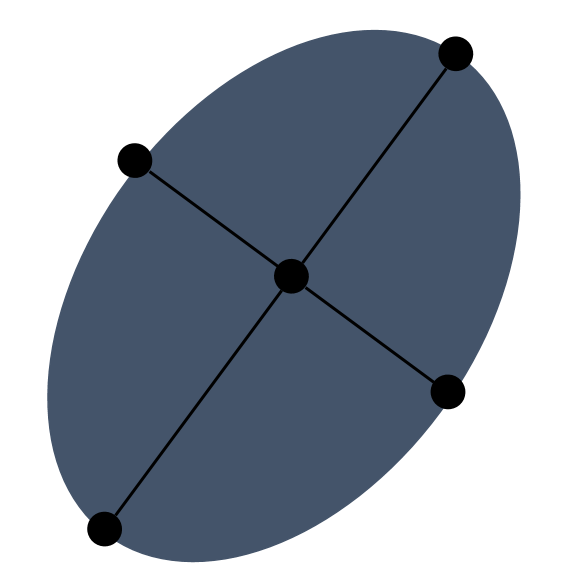
\includegraphics[width=\linewidth]{./ukf1}
	\caption{Initialization of sigma point approximation to the estimate covariance ellipsoid in 2D.}
	\label{fig:ukf1}
	\end{subfigure}
	\hspace{0.04\textwidth}
	\begin{subfigure}[r]{0.35\textwidth}
	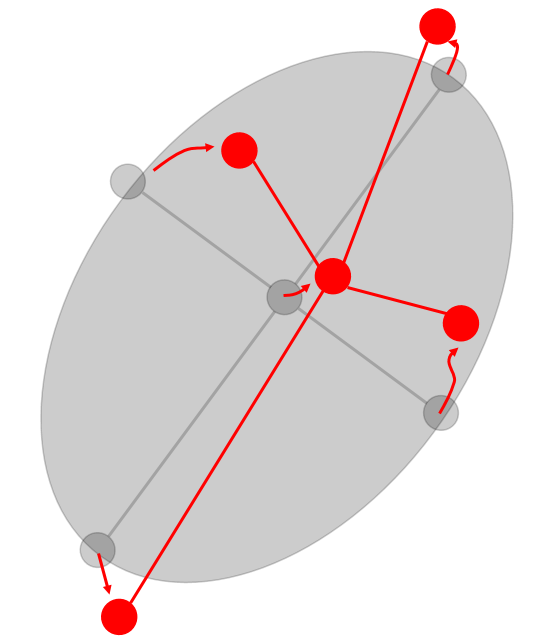
\includegraphics[width=\linewidth]{./ukf2}
	\caption{Propagation of sigma points during the prediction step.}
	\label{fig:ukf2}
	\end{subfigure}
	\\
	\begin{subfigure}[b]{0.35\textwidth}
	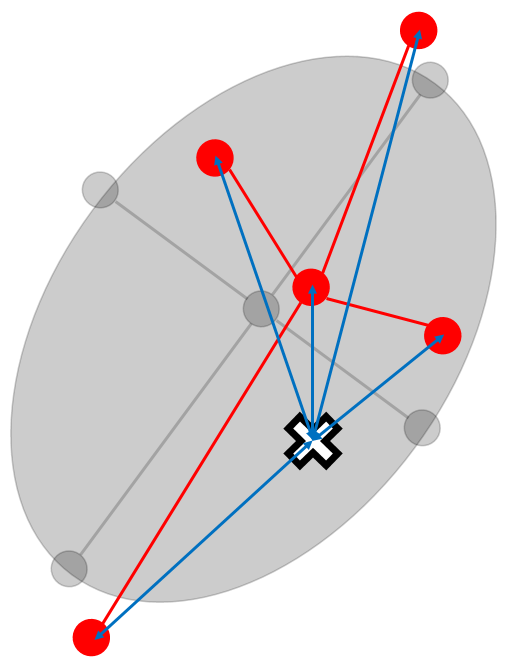
\includegraphics[width=\linewidth]{./ukf3}
	\caption{Computation of the covariance, cross-covariance, and Kalman gain by comparing the prediction sigma points against the measurement.}
	\label{fig:ukf3}
	\end{subfigure}
		\hspace{0.04\textwidth}
	\begin{subfigure}[b]{0.35\textwidth}
	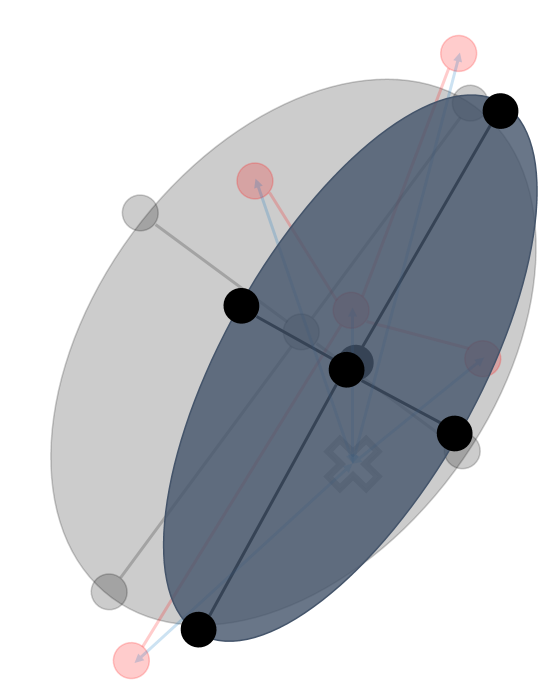
\includegraphics[width=\linewidth]{./ukf4}
	\caption{Re-initialization of sigma points for the next iteration.}
	\label{fig:ukf4}
	\end{subfigure}
	\caption{Graphical summary of the UKF algorithm.}
	\label{fig:ukf_summary}
\end{figure}

A graphical representation of the UKF algorithm is shown in Fig. \ref{fig:ukf_summary} for a 2D random variable.
In the initial step (Fig. \ref{fig:ukf1}), the 2D covariance ellipse is replaced by a particle approximation.
Particles are placed at the mean, and along the positive and negative principal directions.
For the 2D ellipse, this leads to five particles.
Then (Fig. \ref{fig:ukf2}), each of the particles is propagated until the next measurement, using the nonlinear dynamics.
The prediction mean and covariance are determined using a weighted average and weighted variance of the propagated particles.
In Fig. \ref{fig:ukf3}, a measurement is taken (represented by an "X" in the graphic).
The predicted measurement associated with each prediction particle is computed using the nonlinear measurement function.
The measurement is compared against the predicted measurement from the particle values.
The particle predictions are used to approximate a predicted measurement, measurement variance, and cross-covariance between the prediction state and measurement, using weighted means and covariances.
The Kalman gain is computed from these approximations and used to update the prediction mean and variance to a posterior estimate and error variance.
This completes the standard UKF prediction and update cycle.
In Fig. \ref{fig:ukf4}, five new particles are created from the posterior mean and variance, and the filter continues.

A high level-discussion of the UKF has been given; for the full mathematical description, the reader is encouraged to view the appendix.
Now, we turn to a brief comparison of the EKF and UKF, from an application perspective.

Properly implemented, the UKF forms an estimate to a nonlinear process that is at least as good as an EKF estimate.
Due to the higher order approximation implicit in the UKF, it may converge in some cases where an EKF fails.
There is often a tradeoff in terms of computational cost; especially for long state vectors, the EKF algorithm can often exploit matrix sparsity and other linear algebra manipulations to reduce the number of operations required.
The UKF relies upon the nonlinear propagation and measurement expectation of sigma points, and there are fewer opportunities to speed up the computation. 
However, it is true that the UKF and EKF have the same order of computational complexity\cite{wan2000}, making either option much more tractable than methods like particle filters.
The UKF is also somewhat less intuitive for those with a background in analytical estimation.
Finally, although we have not discussed the UKF tuning parameters in this section, they exist and an appropriate choice may not always be obvious.
There don't appear to be well-known automatic or simple heuristic ways to choose those parameters in the literature.

This section has presented the Extended and Unscented Kalman Filters for nonlinear state estimation.
The following section briefly summarizes the overall report.